\documentclass[12pt]{article}
\usepackage{graphicx}
\usepackage[utf8]{inputenc}


\title{List of Style}

\begin{document}
\maketitle



\section{Watercolor}

\subsection*{Description}

This technic use water soluble ink applied with a brush.

\begin{figure}[!ht]
    \begin{center}
        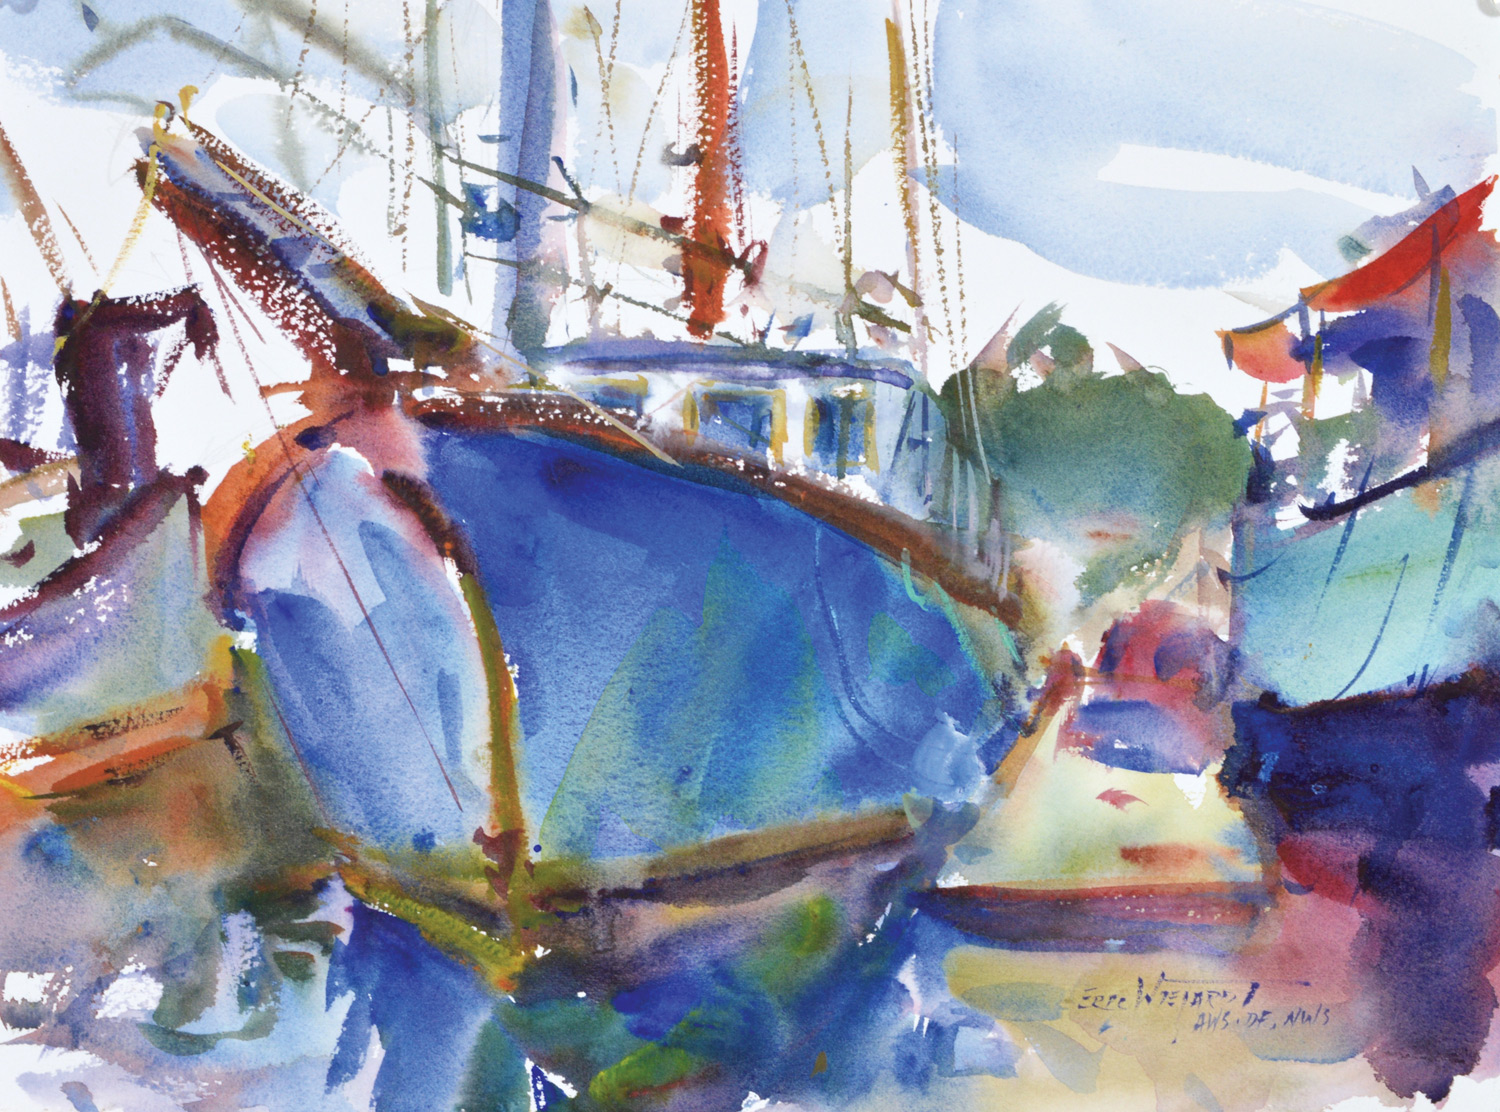
\includegraphics[scale=0.1]{image/watercolor.jpg}
        \caption{example Watercolor}
    \end{center}
\end{figure}

\subsection*{How will we do it}

The splats used will be created with procedural noise in order to not have the same splat. We have to play with the transparency to have this effect of water and wet effect. These splats will be placed by a noise with low frequency and less convolution has possible.

\section{Pointillism}

\subsection*{Description}

This technique consists to paint with only spots of different color.

\begin{figure}[!ht]
    \begin{center}
        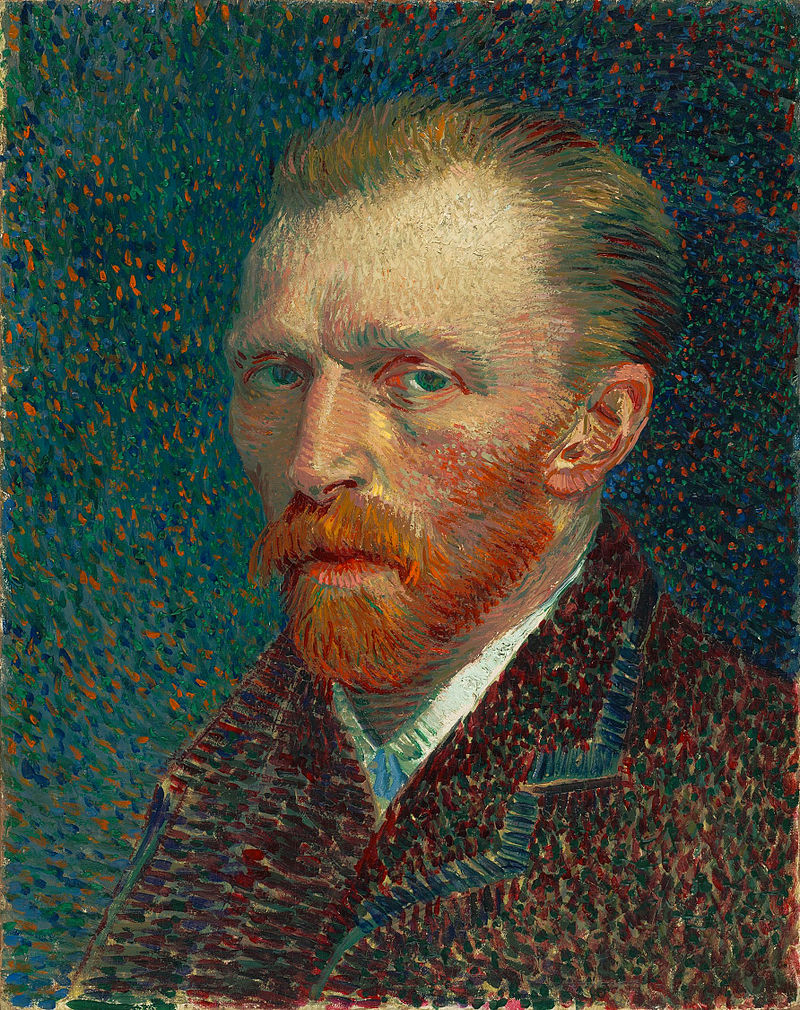
\includegraphics[scale=0.15]{image/VanGogh.jpg}
        \caption{example Pointillism}
    \end{center}
\end{figure}

\subsection*{How will we do it}

The splats will be simple dot or many dots that will placed with a medium/high frequency.

\section{Hatching}

\subsection*{Description}

The technique consists to paint/draw with lines.

\begin{figure}[!ht]
    \begin{center}
        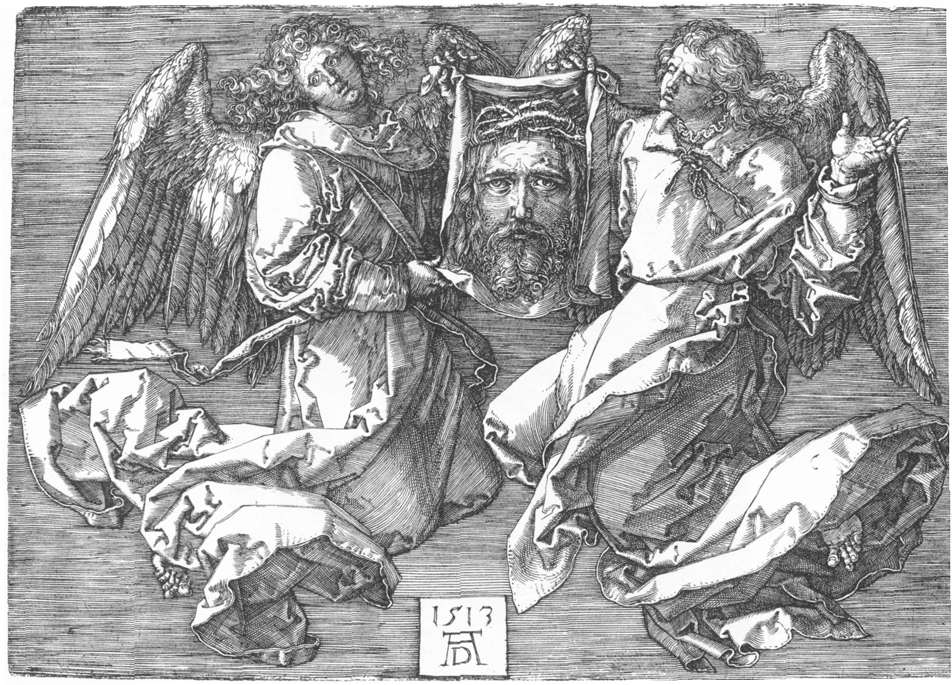
\includegraphics[scale=0.6]{image/hatching.jpg}
        \caption{example Hatching}
    \end{center}
\end{figure}

\subsection*{How will we do it}

The splats will be just one line or many lines. The noise will be at medium/high frequency.


\end{document}
